\documentclass{article}
\usepackage{tikz}
\usepackage{booktabs}

\title{Apuntes de L\'{o}gica Digital}
\date{2023-05-08}
\author{Daniel Araya Rom\'{a}n}

\begin{document}
\maketitle
\newpage

\section*{1. Sistemas Binarios}

\paragraph*{}
\normalsize

\subsection*{1.1 Sistemas Digitales}

En los sistemas digitales electr\'{o}nicos actuales,
las se\~{n}ales emplean s\'{o}lo dos valores discretos
$\rightarrow binarios$. Un d\'{i}gito binario, llamado
\textbf{bit}, que puede tomar los valores 0 y 1.
Un sistema digital es una interconexi\'{o}n de m\'{o}dulos
digitales. Para entender como funciona cada m\'{o}dulo digital,
se necesiatan conocimientos b\'{a}sicos de circuitos digitales
y de su funci\'{o}n l\'{o}gica.

Un lenguaje importante para el dise\~{n}o digital es el \textbf{(HDL,
Hardware Description Language)}. Sirve para simular sistemas digitales
y verificar su funcionamiento antes de crearlos en hardware.
\medskip

\begin{center}
    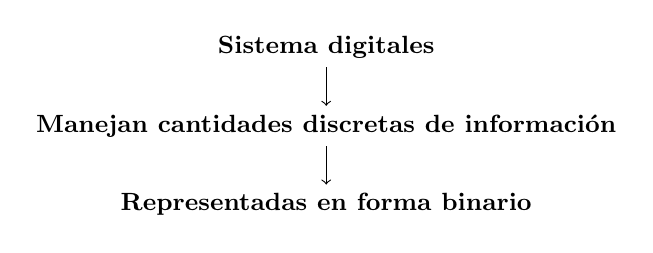
\begin{tikzpicture} 
        \small
        \node (a) at (0,0) {\textbf{Sistema digitales}};
        \node (b) at (0,-1) {\textbf{Manejan cantidades discretas de informaci\'{o}n}};
        \node (c) at (0,-2) {\textbf{Representadas en forma binario}};
        \draw[->] (a) -- (b);
        \draw[->] (b) -- (c);
    \end{tikzpicture}
\end{center}
\medskip

\subsection*{1.2 N\'{u}meros Binarios}

\paragraph*{}
\normalsize

El n\'{u}mero decimal 7392, contiene potencias de 10 que est\'{a}n
impl\'{i}citas en la posici\'{o}n de los coeficientes, e.g:
\medskip

\begin{center}
    $7 \times 10^3 + 3 \times 10^2 + 9 \times 10^1 + 2 \times 10^0$
\end{center}

Un n\'{u}mero con punto decimal se representa con una serie de 
coeficientes, as\'{i}:

\begin{center}
    \large
    $a_5a_4a_3a_2a_1a_0 \cdot a_{-1}a_{-2}a_{-3}$
\end{center}

los coeficientes $a_j$ son cualesquiera de los 10 d\'{i}gitos (0...9);
el valor del sub\'{i}ndice $j$ indica la posici\'{o}n, y la potencia de
10 que se deber\'{a} multplicar ese coeficiente. De modo que:

\begin{center}
    $10^5a_5 + 10^4a_4 + 10^3a_3 + 10^2a_2 + 10^1a_1 + 10^0a_0
     + 10^-1a_{-1} + 10^-2a_{-2} + 10^-3a_{-3}$
\end{center}

El sistema binario es distinto al decimal, sus coeficientes solo pueden
tener 2 valores, 0 o 1. Cada coeficiente $a_j$ se multiplica por $2^j$.
11010.11 es 26.75 en decimal, porque:

\begin{center}
    $1 \times 2^4 + 1 \times 2^3 + 0 \times 2^2 + 1 \times 2^1 + 0 \times 2^0
     + 1 \times 2^{-1} + 1 \times 2^{-2} = 26.75$
\end{center}

En general, un n\'{u}mero expresado en un sistema de base \textbf{r} consiste
en coeficientes que se multiplican por potencias de \textbf{r}:

\begin{center}
    $a_n \cdot r^n + a_{n-1} \cdot r^{n-1} +...+ a_2 \cdot r^2 + a_1 \cdot r 
     + a_0 + a_{-1} \cdot r^{-1} + a_{-2} \cdot r^{-2} +...+ a_{-m} \cdot r^{-m}$
\end{center}

\subsection*{1.4 N\'{u}meros Octales y Hexadecimales}

Las conversiones entre binario, octal y hexadecimal son importantes en las 
computadoras digitales. Puesto que $2^3 = 8$ y $2^4 = 16$, cada d\'{i}gito
octal corresponde a \textbf{tres} d\'{i}gitos binarios, y cada d\'{i}gito
hexadecimal corresponde a \textbf{cuatro} d\'{i}gitos binarios.

$Binario \rightarrow octal$: agrupando los d\'{i}gitos binarios de 3 en 3,
de derecha a izquierda, y reemplazando cada grupo por su equivalente octal.
\begin{center}
    \large
    $(10\,110\,001\,101\,011 \cdot 111\,100\,000\,110)_2 = (26153.7406)_8$
\end{center}

$Binario \rightarrow hexadecimal$: agrupando los d\'{i}gitos binarios de 4 en 4,
de derecha a izquierda, y reemplazando cada grupo por su equivalente hexadecimal.
\begin{center}
    \large
    $(10\,1100\,0110\,1011 \cdot 1111\,0010)_2 = (2C6B.F2)_{16}$
\end{center}

Cuando se habla de binario es m\'{a}s deseable expresarlo en t\'{e}rminos de
n\'{u}meros octales o hexadecimales, porque son m\'{a}s compactos y f\'{a}ciles
de leer. As\'{i} $(111\,111\,111\,111)_2$ este n\'{u}mero en binario de 12 bits,
se puede escribir como $(7777)_8$ en octal o $(FFF)_{16}$ en hexadecimal.

\medskip

\begin{table}[h]
    \centering
    \begin{tabular}{cccc}
        \toprule
        Decimal & Binary & Octal & Hexadecimal \\
        (base 10) & (base 2) & (base 8) & (base 16) \\
        \midrule
        0 & 0000 & 00 & 0 \\
        1 & 0001 & 01 & 1 \\
        2 & 0010 & 02 & 2 \\
        3 & 0011 & 03 & 3 \\
        4 & 0100 & 04 & 4 \\
        5 & 0101 & 05 & 5 \\
        6 & 0110 & 06 & 6 \\
        7 & 0111 & 07 & 7 \\
        8 & 1000 & 10 & 8 \\
        9 & 1001 & 11 & 9 \\
        10 & 1010 & 12 & A \\
        11 & 1011 & 13 & B \\
        12 & 1100 & 14 & C \\
        13 & 1101 & 15 & D \\
        14 & 1110 & 16 & E \\
        15 & 1111 & 17 & F \\
        \bottomrule
    \end{tabular}
    \caption{Numbers in different bases}
    \label{tab:numbers}
\end{table}

\end{document}